\documentclass[aps,prd,twocolumn,superscriptaddress,nofootinbib,floatfix]{revtex4-2}

\usepackage{amsmath,amssymb,amsthm,bm}
\usepackage{graphicx}
\usepackage{booktabs}
\usepackage{tikz}
\usetikzlibrary{decorations.pathmorphing,decorations.markings}
\usepackage[colorlinks=true,linkcolor=blue!60!black,citecolor=blue!60!black,urlcolor=blue!60!black]{hyperref}

\newtheorem{proposition}{Proposition}
\newtheorem{lemma}{Lemma}
\theoremstyle{remark}
\newtheorem*{remark}{Remark}

\newcommand{\Tr}{\mathrm{Tr}}
\newcommand{\Hf}{\mathcal{H}}      % linear field
\newcommand{\G}{\mathcal{G}}
\newcommand{\Hg}{\mathcal{H}_0}    % unbroken group
\newcommand{\p}{\mathfrak{p}}
\newcommand{\h}{\mathfrak{h}}
\newcommand{\ie}{i.e.}
\newcommand{\eg}{e.g.}

\begin{document}

\title{Higgs radial modes and the UV completion of non-linear sigma models}

\author{Giulio Marino}
\email{giulio.marino@phd.unipi.it}
\affiliation{Dipartimento di Fisica ``Enrico Fermi'', Universit\`a di Pisa, Largo B.~Pontecorvo 3, 56127 Pisa, Italy}
\affiliation{INFN, Sezione di Pisa, Largo B.~Pontecorvo 3, 56127 Pisa, Italy}
\affiliation{Dipartimento di Fisica, Sapienza Universit\`a di Roma, Piazzale A.~Moro 2, 00185 Roma, Italy}

\date{\today}

\begin{abstract}
We study the linear UV completions of the non-linear sigma models (NL$\Sigma$Ms) based on the three symmetric cosets realized by fermionic QCD-like theories, $SU(N)\times SU(N)/SU(N)$, $SU(N)/SO(N)$ and $SU(2N)/Sp(2N)$. Treating the three families in a unified way, we identify the minimal linear representation with the complexification of the Jordan algebra of $N\times N$ Hermitian matrices over $\mathbb{R}$, $\mathbb{C}$ and $\mathbb{H}$, and we write the linear sigma model (L$\Sigma$M) in polar coordinates $\Hf=u\,\Phi\, u^{T}$ in a closed form, valid to all orders in the Nambu--Goldstone bosons (NGBs), in which their intrinsic parity is manifest. The radial modes comprise a singlet $h$ and a multiplet $H$ transforming as the NGBs. We prove, uniformly for the three families, that the cancellation of the $\mathcal{O}(E^2)$ growth of NGB scattering amplitudes is equivalent to a matrix identity for the broken generators, which is the Gauss equation of the embedding of the coset into the linear space. From it we derive: (i) a singlet radial mode is necessary in every linear completion, and its coupling is bounded from below by the average sectional curvature of the coset; (ii) a singlet alone suffices if and only if the coset is a sphere, which happens only for $N=2$; (iii) for $N\ge3$ every radial mode of the minimal representation is necessary, and for $N=3$ the radial multiplet $H$ is required in \emph{any} linear completion. We compare this approach with a purely group-theoretical construction, derive tree-level unitarity bounds on the radial-mode masses, and comment on the phenomenology of the radial modes in electroweak symmetry breaking.
\end{abstract}

\maketitle

%=====================================================================
\section{Introduction}
\label{sec:intro}
%=====================================================================

Non-linear sigma models describe the low-energy dynamics of the Nambu--Goldstone bosons (NGBs) arising from the spontaneous breaking of a global symmetry $\G\to\Hg$~\cite{Nambu:1960xd,Goldstone:1961eq,Goldstone:1962es}. The NGBs $\pi^a$ are coordinates on the coset $\G/\Hg$, and the most general two-derivative Lagrangian is fixed by the Callan--Coleman--Wess--Zumino (CCWZ) construction~\cite{Coleman:1969sm,Callan:1969sn} up to the decay constant $f$,
\begin{equation}
\mathcal{L}=\tfrac12\, g_{ab}(\pi)\,\partial_\mu\pi^a\partial^\mu\pi^b+\dots ,
\label{eq:NLSMgeneric}
\end{equation}
where $g_{ab}$ is the $\G$-invariant metric on the coset. Since the interactions carry derivatives, NGB scattering amplitudes grow with energy, $\mathcal{A}\sim E^2/f^2$~\cite{Weinberg:1966kf}, and perturbative unitarity is lost at $\Lambda\sim 4\pi f$. Above this scale the theory either becomes strongly coupled, as in QCD and in technicolor, or new weakly coupled degrees of freedom enter. The linear sigma model (L$\Sigma$M) of Gell-Mann and L\'evy~\cite{GellMann:1960np} is the prototype of the second possibility: the NGBs are embedded in a linear representation of $\G$ together with additional ``radial'' modes, the theory is renormalizable, and the $E^2$ growth is cancelled by radial-mode exchange. In the Standard Model (SM) the Higgs boson plays precisely this role for the would-be NGBs eaten by the $W$ and $Z$~\cite{Lee:1977eg,Dicus:1973gbw}.\footnote{By ``UV completion'' we mean a weakly coupled extension valid well above $4\pi f$; the renormalization-group evolution of the quartic couplings may eventually drive the L$\Sigma$M to strong coupling (Landau pole), as for the SM Higgs sector.}

In this paper we study the linear completions of the three classes of NL$\Sigma$Ms that are realized by asymptotically free gauge theories with $N$ Dirac or $2N$ Weyl fermions in complex, real or pseudo-real representations of the gauge group, respectively~\cite{Peskin:1980gc,Preskill:1980mz,Dimopoulos:1980hn,Dimopoulos:1981xc,Kogut:2000ek}:
\begin{equation}
\frac{SU(N)\times SU(N)}{SU(N)},\qquad \frac{SU(N)}{SO(N)},\qquad \frac{SU(2N)}{Sp(2N)} .
\label{eq:cosets}
\end{equation}
These patterns are the basis of technicolor and of fundamental composite Higgs models~\cite{Kaplan:1983fs,Agashe:2004rs,Contino:2010rs,Panico:2015jxa,Bellazzini:2014yua,Galloway:2010bp,Barnard:2013zea,Ferretti:2013kya,Ferretti:2014qta,Cacciapaglia:2014uja,Cacciapaglia:2020kgq}, and their chiral Lagrangians have been studied in detail, including the general decomposition of the meson--meson scattering amplitudes~\cite{Gasser:1983yg,Gasser:1984gg,Chivukula:1992gi,Splittorff:2001fy,Splittorff:2002xn,Bijnens:2009qm,Bijnens:2011fm}. Linear sigma models with more than two flavors have a long history in hadron physics~\cite{Schechter:1971qa,Pisarski:1983ms,Lenaghan:2000ey,Fariborz:2005gm,Parganlija:2012fy}, and linear models of the composite Higgs have been used as weakly coupled benchmarks~\cite{Barbieri:2007bh,Alanne:2014kea,Gertov:2015xma}.

For $N=2$ the three cosets are spheres, $SU(2)\times SU(2)/SU(2)\simeq SO(4)/SO(3)$, $SU(2)/SO(2)\simeq SO(3)/SO(2)$ and $SU(4)/Sp(4)\simeq SO(6)/SO(5)$, and a single real singlet radial mode is sufficient: the completion is the $O(n)$ vector model. For $N\geq 3$ the smallest linear representation of $\G$ containing the NGBs contains more radial modes than a singlet, and the question we address is: \emph{which radial modes are actually required to restore perturbative unitarity, and is the answer specific to the chosen representation?}

There are two complementary ways to approach this question. The first one is group theoretical: one looks for a representation of $\G$ that contains the NGB representation of $\Hg$ and a $\Hg$-singlet direction for the vacuum; any renormalizable L$\Sigma$M built on it is automatically well behaved at high energy. The second one, which we develop here, starts from the scattering amplitudes of the NL$\Sigma$M: requiring the cancellation of their $E^2$ growth gives sum rules on the couplings of the radial modes, which are representation independent. We show that these sum rules are the Gauss equation of the embedding of $\G/\Hg$ into the linear field space, in line with the geometric formulation of scalar effective theories~\cite{Alonso:2015fsp,Alonso:2016oah,Nagai:2019tgi,Falkowski:2019tft,Cohen:2020xca,Cohen:2021ucp} and with the Higgs sum rules of Refs.~\cite{Gunion:1990kf,Falkowski:2012vh}. The sum rules tell us which radial modes are necessary in \emph{any} linear completion, while group theory provides the minimal completion that saturates them.

The main results of this work are the following.
\begin{itemize}
\item[(1)] We give a unified construction of the minimal L$\Sigma$M for the three families. The linear field lives in the complexification of the Jordan algebra $J_N(\mathbb{K})$ of $N\times N$ Hermitian matrices over $\mathbb{K}=\mathbb{C},\mathbb{R},\mathbb{H}$; the radial modes are a singlet $h$ and a multiplet $H^a$ in the same $\Hg$-representation as the NGBs (Sec.~\ref{sec:group}).
\item[(2)] Using the polar parametrization $\Hf=u\Phi u^T$ (or $u\Phi u$) with $u$ unitary and $\Phi$ Hermitian, we write the L$\Sigma$M Lagrangian in closed form, Eq.~\eqref{eq:master}, valid to all orders in the NGB fields. Intrinsic parity of the NGBs is manifest and is a symmetry of the L$\Sigma$M (Sec.~\ref{sec:LSM}).
\item[(3)] We prove, for the three families at once, that the tree-level $\pi\pi\to\pi\pi$ amplitude is bounded at high energy, with the exact result Eq.~\eqref{eq:Afull}, and that the cancellation follows from the matrix identity of Lemma~\ref{lem:identity} (Sec.~\ref{sec:scattering}).
\item[(4)] From the Gauss equation we derive model-independent statements (Propositions~\ref{prop:singlet}--\ref{prop:rigidity}): a singlet radial mode is always necessary; a singlet alone suffices if and only if the coset is a sphere, \ie\ $N=2$; for $N\ge 3$ all radial modes of the minimal representation are necessary; for $N=3$ any linear completion must contain the radial multiplet $H$, with couplings at least as large as in the minimal model (Secs.~\ref{sec:geometry} and~\ref{sec:beyond}).
\item[(5)] We derive tree-level unitarity bounds on the radial-mode masses, Eq.~\eqref{eq:unitarity_singlet} and Fig.~\ref{fig:unitarity}, and discuss the phenomenology of the radial modes in electroweak symmetry breaking (Secs.~\ref{sec:unitarity} and~\ref{sec:pheno}).
\end{itemize}

%=====================================================================
\section{Symmetric cosets and linear completions}
\label{sec:geometry}
%=====================================================================

\subsection{The non-linear sigma model}

Let $\mathfrak{g}=\h\oplus\p$ be the decomposition of the Lie algebra of $\G$ into the unbroken subalgebra $\h$ and its orthogonal complement $\p$. All the cosets in Eq.~\eqref{eq:cosets} are \emph{symmetric}: there is an automorphism $\mathcal{R}$ of $\mathfrak g$ (the grading) with $\mathcal{R}(T^I)=T^I$ for $T^I\in\h$ and $\mathcal{R}(X^a)=-X^a$ for $X^a\in\p$, so that
\begin{equation}
[\h,\h]\subset\h,\qquad [\h,\p]\subset\p,\qquad [\p,\p]\subset\h .
\label{eq:symmetric}
\end{equation}
In the three cases of interest $\G$ is realized by $n\times n$ unitary matrices, with $n=N,N,2N$, and it is convenient to include an extra $U(1)$ factor, under which the linear field of Sec.~\ref{sec:group} has unit charge. Its NGB, $\eta\equiv\pi^0$, corresponds to the generator $X^0=\mathbb{1}/\sqrt{2n}$. We use capital indices $A,B,\ldots=0,1,\dots,D$ for the extended set of broken generators, lower-case indices $a,b,\ldots=1,\dots,D$ for the non-abelian NGBs, and $I,J,\ldots$ for $\h$. The normalization is $\Tr(X^AX^B)=\tfrac12\delta^{AB}$, $\Tr(T^IT^J)=\tfrac12\delta^{IJ}$, and
\begin{equation}
[X^A,X^B]=i f^{ABI}T^I .
\label{eq:fdef}
\end{equation}

The NGB field is $u(\pi)=\exp(i\pi^AX^A/f)$. Under $g\in\G$, $u\to g\,u\,k^{-1}(g,\pi)$ with $k\in\Hg$ (for the chiral case $u\to L\,u\,k^\dagger=k\,u\,R^\dagger$). The Maurer--Cartan form decomposes into a covariant part $d_\mu\in\p$ and a connection $E_\mu\in\h$, $u^{-1}\partial_\mu u=i(d_\mu+E_\mu)$ (for the chiral case $u^\dagger\partial_\mu u=i(d_\mu+E_\mu)$, $u\partial_\mu u^\dagger=i(-d_\mu+E_\mu)$), with
\begin{align}
d_\mu &=\frac{\partial_\mu\pi^AX^A}{f}-\frac{1}{6f^3}\big[\pi\!\cdot\! X,[\pi\!\cdot\! X,\partial_\mu\pi\!\cdot\! X]\big]+\mathcal{O}(\pi^5),\nonumber\\
E_\mu &=\frac{1}{2f^2}f^{ABI}\pi^A\partial_\mu\pi^BT^I+\mathcal{O}(\pi^4).
\label{eq:dE}
\end{align}
The leading-order NL$\Sigma$M Lagrangian is
\begin{align}
\mathcal{L}_{\rm NL\Sigma M}&=f^2\,\Tr(d_\mu d^\mu)\nonumber\\
&=\tfrac12(\partial_\mu\pi^A)^2\nonumber\\&\quad-\frac{1}{6f^2}f^{ABI}f^{CDI}\pi^A\partial_\mu\pi^B\pi^C\partial^\mu\pi^D+\mathcal{O}(\pi^6).
\label{eq:LNLSM}
\end{align}
For the chiral coset this coincides with the familiar $\tfrac{f^2}{4}\Tr(\partial_\mu\Sigma^\dagger\partial^\mu\Sigma)$, $\Sigma=u^2$. The $\eta$ is free at this order, since $f^{0BI}=0$. The grading acts on the NGBs as $\pi^A\to-\pi^A$, \ie\ $d_\mu\to-d_\mu$ and $E_\mu\to E_\mu$; it is the intrinsic parity of the NGBs and is broken only by the Wess--Zumino--Witten term~\cite{Wess:1971yu,Witten:1983tw}, which arises at higher order in the derivative expansion.

For massless NGBs, the tree-level amplitude $\mathcal{A}(\pi^a\pi^b\to\pi^c\pi^d)$ obtained from Eq.~\eqref{eq:LNLSM} reads
\begin{equation}
\mathcal{A}_{\rm NL\Sigma M}=-\frac{1}{f^2}\Big[t\,f^{adI}f^{bcI}+u\,f^{acI}f^{bdI}\Big],
\label{eq:ANLSM}
\end{equation}
with $s=(p_a+p_b)^2$, $t=(p_a-p_c)^2$, $u=(p_a-p_d)^2$. The tensor $f^{abI}f^{cdI}/f^2$ is, up to sign conventions, the Riemann tensor of the coset at the origin, so the $E^2$ growth is controlled by the curvature of $\G/\Hg$~\cite{Alonso:2016oah,Cohen:2021ucp}. For $SU(2)\times SU(2)/SU(2)$, where $f^{abI}=\epsilon^{abI}$, this is Weinberg's amplitude $\mathcal{A}=\delta^{ab}\delta^{cd}s/f^2+\delta^{ac}\delta^{bd}t/f^2+\delta^{ad}\delta^{bc}u/f^2$~\cite{Weinberg:1966kf}. The decomposition of Eq.~\eqref{eq:ANLSM} into invariant flavor structures is given for the three families in Refs.~\cite{Chivukula:1992gi,Bijnens:2011fm}.

\subsection{Linear completions and the Gauss equation}
\label{sec:Gauss}

Consider now a generic renormalizable completion: real scalars $\phi$ in a (possibly reducible) orthogonal representation of $\G$, with Lagrangian $\tfrac12(\partial\phi)^2-V(\phi)$ and a vacuum $v$ whose stabilizer is $\Hg$. Writing $\phi=U(\pi)(v+\rho)$, where $U(\pi)$ represents $u(\pi)$ and $\rho$ spans the directions orthogonal to the orbit (the radial modes), the kinetic term contains the NL$\Sigma$M~\eqref{eq:LNLSM}, plus the cubic couplings
\begin{equation}
\mathcal{L}\supset \frac{1}{f}\,g^r_{ab}\,\rho^r\,\partial_\mu\pi^a\partial^\mu\pi^b ,\qquad g^r_{ab}=g^r_{ba}.
\label{eq:cubicgeneric}
\end{equation}
Geometrically, $g^r_{ab}$ is the second fundamental form of the orbit $\G\cdot v\simeq\G/\Hg$ in the field space, \ie\ the normal component of $\{t^a,t^b\}v$, where $t^a$ are the broken generators in the representation of $\phi$~\cite{Alonso:2016oah,Cohen:2021ucp}. Radial modes with masses $m_r$ contribute to $\pi\pi\to\pi\pi$ through $s$, $t$ and $u$-channel exchange:
\begin{equation}
\begin{split}
\mathcal{A}_\rho=-\frac{1}{f^2}\sum_r\bigg[&g^r_{ab}g^r_{cd}\frac{s^2}{s-m_r^2}+g^r_{ac}g^r_{bd}\frac{t^2}{t-m_r^2}\\
&+g^r_{ad}g^r_{bc}\frac{u^2}{u-m_r^2}\bigg].
\end{split}
\label{eq:Arho}
\end{equation}
In Cartesian coordinates $\phi$ the theory has no derivative interactions and all tree-level two-to-two amplitudes are bounded at high energy; since the $S$-matrix is invariant under field redefinitions, the $\mathcal{O}(E^2)$ terms of $\mathcal{A}_{\rm NL\Sigma M}+\mathcal{A}_\rho$ must cancel. Using $s^2/(s-m^2)=s+m^2+\mathcal{O}(m^4/s)$ and $s+t+u=0$, the cancellation is equivalent to
\begin{equation}
\boxed{\;f^{abI}f^{cdI}=\sum_r\left(g^r_{ac}g^r_{bd}-g^r_{ad}g^r_{bc}\right),\;}
\label{eq:Gauss}
\end{equation}
which is the Gauss equation relating the intrinsic curvature of the coset to the extrinsic curvature of its embedding~\cite{KobayashiNomizu}, the ambient space being flat. Equation~\eqref{eq:Gauss} is the content of the statement that ``the radial modes unitarize NGB scattering'', and generalizes the familiar sum rules for Higgs couplings~\cite{Gunion:1990kf,Falkowski:2012vh}. It holds for any linear completion and can be used to constrain the radial content without specifying the representation. Two consequences are immediate.

\begin{proposition}[the singlet is necessary]
\label{prop:singlet}
Let the NGBs $\pi^a$ transform in an irreducible representation of $\Hg$ of dimension $D$. Every linear completion contains $\Hg$-singlet radial modes $\rho^r$, with couplings $g^r_{ab}=g_r\delta_{ab}$ satisfying
\begin{equation}
\sum_{r\in\text{singlets}}g_r^2\;\geq\;\bar K\equiv\frac{f^{abI}f^{abI}}{D(D-1)} .
\label{eq:singletbound}
\end{equation}
\end{proposition}
\begin{proof}
Contract Eq.~\eqref{eq:Gauss} with $\delta_{ac}\delta_{bd}$. The left-hand side is the scalar curvature, $f^{abI}f^{abI}>0$. Decomposing $g^r=\frac{\Tr g^r}{D}\mathbb{1}+\hat g^r$, the right-hand side is $\sum_r[(\Tr g^r)^2\frac{D-1}{D}-\Tr(\hat g^r)^2]$. By $\Hg$-invariance $\Tr g^r\neq0$ only for singlets, for which $\Tr g^r=Dg_r$. Hence $D(D-1)\sum_{\rm singlets}g_r^2=f^{abI}f^{abI}+\sum_r\Tr(\hat g^r)^2\geq f^{abI}f^{abI}$.
\end{proof}
$\bar K$ is the average sectional curvature of the coset in units of $f^{-2}$. For the three families
\begin{equation}
\bar K=\frac{N}{N^2-2},\qquad \frac{N}{N^2+N-4},\qquad \frac{N}{2N^2-N-2},
\label{eq:Kbar}
\end{equation}
respectively. The isotropic average of the curvature, $f^{abI}f^{cdI}\to\bar K(\delta_{ac}\delta_{bd}-\delta_{ad}\delta_{bc})$, is exact only for spaces of constant curvature.

\begin{proposition}[singlets alone suffice iff the coset is a sphere]
\label{prop:sphere}
A completion in which only $\Hg$-singlet radial modes couple to $\pi\pi$ exists if and only if $f^{abI}f^{cdI}\propto\delta_{ac}\delta_{bd}-\delta_{ad}\delta_{bc}$, \ie\ the coset has constant curvature. For the cosets~\eqref{eq:cosets} this happens only for $N=2$.
\end{proposition}
\begin{proof}
With singlets only, $g^r_{ab}=g_r\delta_{ab}$ and Eq.~\eqref{eq:Gauss} gives $f^{abI}f^{cdI}=(\sum_rg_r^2)(\delta_{ac}\delta_{bd}-\delta_{ad}\delta_{bc})$, \ie\ constant sectional curvature $\sum_r g_r^2$; conversely the $O(D+1)$ vector model completes a sphere. The cosets~\eqref{eq:cosets} have rank $N-1$~\cite{Helgason}: $\p$ contains an abelian subspace of dimension $N-1$, made of diagonal matrices (of the form ${\rm diag}(\Lambda,\Lambda)$ in the symplectic case). For $N\geq3$ two commuting generators $X^a,X^b$ span a plane of vanishing sectional curvature, $f^{abI}f^{abI}=0$ (no sum), while non-commuting pairs give a positive one. Hence the curvature is not constant.
\end{proof}

We have checked numerically that for $N=3,4$ the sectional curvatures of the three families range in $[0,1]$, $[0,1]$ and $[0,\tfrac12]$ respectively, while for $N=2$ they are constant (equal to $1$, $1$ and $\tfrac12$). Proposition~\ref{prop:sphere} explains why $N=2$ is special: for $N\ge 3$ at least one non-singlet radial multiplet must couple to the NGBs, whatever representation of $\G$ is used.

%=====================================================================
\section{Group theory: the minimal linear representations}
\label{sec:group}
%=====================================================================

\begin{table*}[t]
\caption{Minimal linear completions of the three cosets. $n$ is the size of the matrix $\Hf$, $D_{\mathbb{R}}$ its number of real components. The NGBs $\pi^a$ and the radial multiplet $H^a$ transform in the same representation of $\Hg$, of dimension $D$; the singlets are the $U(1)$ NGB $\eta$ and the radial singlet $h$. For $N=2$ the multiplet decouples from $\pi\pi$ scattering ($d^{abc}=0$) and the cosets are the spheres $S^3$, $S^2$ and $S^5$.}
\label{tab:reps}
{\small
\begin{ruledtabular}
\begin{tabular}{lccccccc}
Coset & $\Hf$ & $\G$ action & $\langle\Hf\rangle$ & $n$ & $D_{\mathbb{R}}$ & $\pi^a$, $H^a$ ($D$) & Jordan algebra $\p$ \\
\hline
$\frac{SU(N)_L\times SU(N)_R\times U(1)}{SU(N)_V}$ & $\Hf\in\mathrm{Mat}(N,\mathbb{C})$ & $e^{i\alpha}L\,\Hf R^\dagger$ & $\frac{f}{\sqrt2}\mathbb{1}$ & $N$ & $2N^2$ & adjoint, $N^2-1$ & $J_N(\mathbb{C})$ \\
$\frac{SU(N)\times U(1)}{SO(N)}$ & $\Hf=\Hf^T$ & $e^{i\alpha}V\Hf V^T$ & $\frac{f}{\sqrt2}\mathbb{1}$ & $N$ & $N(N+1)$ & sym.\ traceless, $\frac{N(N+1)}{2}{-}1$ & $J_N(\mathbb{R})$\\
$\frac{SU(2N)\times U(1)}{Sp(2N)}$ & $\Hf=-\Hf^T$ & $e^{i\alpha}V\Hf V^T$ & $\frac{f}{\sqrt2}\Omega$ & $2N$ & $2N(2N-1)$ & antisym.\ $\Omega$-traceless, $2N^2{-}N{-}1$ & $J_N(\mathbb{H})$
\end{tabular}
\end{ruledtabular}}
\end{table*}

The group-theoretical approach is to find a representation of $\G$ that contains a $\Hg$-singlet (the vacuum direction) and the NGB representation of $\Hg$ in its tangent space. For the three families the minimal choice is a complex matrix $\Hf$ in the representations listed in Table~\ref{tab:reps}: the bifundamental for the chiral coset, the two-index symmetric for $SU(N)/SO(N)$ and the two-index antisymmetric for $SU(2N)/Sp(2N)$, with $\Omega=\left(\begin{smallmatrix}0&\mathbb{1}_N\\-\mathbb{1}_N&0\end{smallmatrix}\right)$~\cite{Peskin:1980gc,Preskill:1980mz,Dimopoulos:1981xc,Kogut:2000ek}. Since these representations are complex for $N\ge3$ (and the $U(1)$ charge makes them complex also for $N=2$), no reality condition can reduce the number of fields. For $N\ge3$ they are the smallest representations with the required vacuum. For $SU(N)\times SU(N)$, for instance, a representation $(R_1,R_2)$ contains an $SU(N)_V$ singlet only if $R_2\simeq\bar R_1$.

A unifying structure emerges by looking at the broken generators. In the three cases $\p$, extended by the identity $X^0$, is closed under anticommutation,
\begin{equation}
\{X^A,X^B\}=d^{ABC}X^C,\quad d^{ABC}=2\,\Tr\big(\{X^A,X^B\}X^C\big),
\label{eq:ddef}
\end{equation}
\ie\ $\p\oplus\mathbb{R}\mathbb{1}$ is a Jordan algebra~\cite{Jordan:1933vh,FarautKoranyi}: the Hermitian matrices $J_N(\mathbb{C})$ for the chiral coset, the real symmetric matrices $J_N(\mathbb{R})$ for $SU(N)/SO(N)$, and the $2N\times2N$ Hermitian matrices satisfying $X^T\Omega=\Omega X$, isomorphic to the quaternionic Hermitian matrices $J_N(\mathbb{H})$, for $SU(2N)/Sp(2N)$. The linear field $\Hf$ is an element of the complexification of $J_N(\mathbb K)$ (times $\Omega$ in the symplectic case), and the cosets~\eqref{eq:cosets} are the compact symmetric spaces naturally associated with these Jordan algebras. The symbols $d^{ABC}$ are the generalization of the $U(N)$ $d$-symbols~\cite{Haber:2019sgz}: $d^{AB0}=\sqrt{2/n}\,\delta^{AB}$, and $d^{acd}d^{bcd}=C_d\,\delta^{ab}$ with
\begin{equation}
C_d=\frac{N^2-4}{N},\quad \frac{(N+4)(N-2)}{2N},\quad \frac{(N+1)(N-2)}{N}
\label{eq:Cd}
\end{equation}
for the three families. For $N=2$ the Jordan algebra is a spin factor: every traceless element squares to a multiple of the identity, so $d^{abc}=0$ for $a,b,c\geq1$. This is the algebraic origin of the simplification of the $N=2$ cases.

Decomposing $\Hf$ into its ``Hermitian'' and ``anti-Hermitian'' parts with respect to $J_N(\mathbb{K})$ shows that the radial modes span a second copy of $J_N(\mathbb{K})$: a singlet $h$ and a multiplet $H^a$ transforming under $\Hg$ exactly as the NGBs $\pi^a$,
\begin{equation}
D_{\mathbb R}=\underbrace{(D+1)}_{\pi^a,\;\eta}+\underbrace{(D+1)}_{H^a,\;h}.
\label{eq:counting}
\end{equation}
Group theory thus fixes the candidate radial content. It does not tell us, however, whether each radial mode is \emph{dynamically} required, whether a different (possibly reducible and smaller) representation could do the same job, or which radial modes unitarize which channels. These questions are answered by the Gauss equation~\eqref{eq:Gauss} and by the explicit amplitudes of Secs.~\ref{sec:scattering} and~\ref{sec:beyond}.

%=====================================================================
\section{The linear sigma model in polar coordinates}
\label{sec:LSM}
%=====================================================================

\subsection{Parametrization and parity}

Any complex matrix admits a polar decomposition into a unitary and a Hermitian factor; for complex symmetric (antisymmetric) matrices the corresponding statement is the Takagi factorization~\cite{Takagi:1924,HornJohnson}. Around the vacuum we parametrize the three linear fields as
\begin{equation}
\sqrt2\,\Hf=u\,\Phi\,u,\quad u\,\Phi\,u^T,\quad u\,\Phi\,\Omega\,u^T ,
\label{eq:polar}
\end{equation}
with $u=\exp(i\pi^AX^A/f)$ and
\begin{equation}
\Phi=f\,\mathbb{1}+2\rho^AX^A=\Big(f+\sqrt{\tfrac{2}{n}}\,h\Big)\mathbb{1}+2H^aX^a ,
\label{eq:Phi}
\end{equation}
where $\rho^0\equiv h$ and $\rho^a\equiv H^a$. For the second family $u^T=u$, since the broken generators are symmetric. The conditions $X^T\Omega=\Omega X$ ensure that $\Phi\Omega$ is antisymmetric in the third family. Equation~\eqref{eq:Phi} is the precise version, for the three families at once, of the parametrization $\Hf=u\phi u$ with $u$ unitary and $\phi$ Hermitian. Under $\G$, $u\to g\,u\,k^{-1}$ and $\Phi\to k\,\Phi\,k^{-1}$, so the radial modes transform linearly under the compensating $\Hg$ transformation. The counting matches Eq.~\eqref{eq:counting}.

The grading $\pi^A\to-\pi^A$ maps $u\to u^\dagger$, and therefore acts on the linear field as
\begin{equation}
\Hf\to\Hf^\dagger,\qquad \Hf\to\Hf^*,\qquad \Hf\to\Omega^{-1}\Hf^*\Omega,
\label{eq:parity}
\end{equation}
for the three families respectively, as follows from $u^*=u^\dagger$ for the second family and from $X^T=\Omega X\Omega^{-1}$ for the third. In the symplectic case the transformation is complex conjugation followed by the $Sp(2N)$ element $\Omega^{-1}$, under which $\Hf\to\Omega^{-1}\Hf(\Omega^{-1})^T$. The transformation~\eqref{eq:parity} leaves invariant the kinetic term $\tfrac12\Tr(\partial\Hf^\dagger\partial\Hf)$ and every potential built out of $\Tr[(\Hf^\dagger\Hf)^k]$, as well as $\det\Hf+{\rm h.c.}$ (or ${\rm Pf}\,\Hf+{\rm h.c.}$) with a real coefficient. Intrinsic parity is therefore \emph{not} an accidental symmetry of the NL$\Sigma$M: it is the symmetry $\Hf\to\Hf^\dagger$ ($\Hf\to\Hf^*$) of the L$\Sigma$M, which in the parametrization~\eqref{eq:polar} acts as $\pi\to-\pi$ with $h$, $H^a$ even. Consequently no vertex with an odd number of NGBs is generated. It can be broken only by a complex phase in the determinant (Pfaffian) term, a $\theta$-like parameter, while the WZW term arises from the anomalies of the underlying fermionic theory and is absent in the renormalizable L$\Sigma$M.

\subsection{Closed-form Lagrangian}

The L$\Sigma$M Lagrangian is
\begin{equation}
\mathcal{L}=\tfrac12\Tr\big(\partial_\mu\Hf^\dagger\partial^\mu\Hf\big)-V(\Hf) .
\label{eq:LSM}
\end{equation}
Inserting Eq.~\eqref{eq:polar} and using the Maurer--Cartan decomposition, one finds $\sqrt2\,u^{-1}\partial_\mu\Hf\,(u^T)^{-1}=\big(i\{d_\mu,\Phi\}+\nabla_\mu\Phi\big)\,(\Omega)$, with $\nabla_\mu\Phi=\partial_\mu\Phi+i[E_\mu,\Phi]$ the CCWZ covariant derivative (for the chiral case $u^{-1}$ and $(u^T)^{-1}$ are replaced by $u^\dagger$ on both sides). Since $\{d_\mu,\Phi\}$ and $\nabla_\mu\Phi$ are Hermitian, the cross terms cancel in the trace, and we obtain the exact result
\begin{equation}
\boxed{\;\mathcal{L}=\tfrac14\Tr\big[(\nabla_\mu\Phi)^2\big]+\tfrac14\Tr\big[\{d_\mu,\Phi\}^2\big]-V(\Phi),\;}
\label{eq:master}
\end{equation}
valid to all orders in $\pi$ and for the three families. The potential depends only on $\Phi$, because $\Tr[(\Hf^\dagger\Hf)^k]=2^{-k}\Tr\Phi^{2k}$. Equation~\eqref{eq:master} makes several properties manifest. For $\Phi=f\mathbb{1}$ it reduces to the NL$\Sigma$M~\eqref{eq:LNLSM}. It is even under $d_\mu\to-d_\mu$, \ie\ under intrinsic parity. The radial modes couple to the NGBs only through the $\Hg$-covariant objects $d_\mu$ and $E_\mu$, so all NGB interactions are derivative ones, as required by the Goldstone theorem.

Expanding Eq.~\eqref{eq:master} with Eqs.~\eqref{eq:dE} and~\eqref{eq:Phi}, the terms relevant for two-to-two scattering are
\begin{align}
\mathcal{L}&=\tfrac12(\partial\pi^A)^2+\tfrac12(\partial\rho^A)^2-\frac{1}{6f^2}f^{ABI}f^{CDI}\pi^A\partial\pi^B\!\cdot\pi^C\partial\pi^D\nonumber\\
&+\frac{1}{f}\,d^{ABC}\rho^C\,\partial\pi^A\!\cdot\partial\pi^B\nonumber\\
&+\frac{1}{2f^2}d^{ACE}d^{BDE}\rho^C\rho^D\,\partial\pi^A\!\cdot\partial\pi^B\nonumber\\
&-\frac{1}{2f^2}f^{ABI}f^{CEI}\pi^A\partial\pi^B\!\cdot\rho^C\partial\rho^E-V+\dots ,
\label{eq:expanded}
\end{align}
where the dots denote terms with five or more fields. The explicit form in terms of $h$, $\eta$, $H^a$ and $\pi^a$ is given in Appendix~\ref{app:lagrangian}. In particular, the cubic couplings~\eqref{eq:cubicgeneric} are $g^C_{AB}=d^{ABC}$, \ie\ the second fundamental form is the Jordan product:
\begin{equation}
\begin{split}
\mathcal{L}_3={}&\frac{1}{f}\sqrt{\frac{2}{n}}\,h\,\big[(\partial\pi^a)^2+(\partial\eta)^2\big]+\frac1f d^{abc}H^c\,\partial\pi^a\!\cdot\partial\pi^b\\
&+\frac{2}{f}\sqrt{\frac{2}{n}}\,H^a\,\partial\pi^a\!\cdot\partial\eta .
\end{split}
\label{eq:cubic}
\end{equation}
We have verified Eqs.~\eqref{eq:master} and~\eqref{eq:expanded} numerically, by comparing them with a direct evaluation of Eq.~\eqref{eq:LSM} for random field configurations for $N=2,3,4$ in the three families.

\subsection{Potential and spectrum}

The most general renormalizable potential invariant under $\G$ (including the $U(1)$) is
\begin{equation}
V=-\frac{\mu^2}{2}\Tr(\Hf^\dagger\Hf)+\frac{\lambda_1}{4}\big[\Tr(\Hf^\dagger\Hf)\big]^2+\frac{\lambda_2}{4}\Tr\big[(\Hf^\dagger\Hf)^2\big].
\label{eq:V}
\end{equation}
For $\lambda_2>0$ and $n\lambda_1+\lambda_2>0$ the minimum is at $\Phi=f\mathbb{1}$, \ie\ along the $\Hg$-invariant direction of Table~\ref{tab:reps}, with
\begin{equation}
\begin{split}
&f^2=\frac{2\mu^2}{n\lambda_1+\lambda_2},\\
&m_h^2=(n\lambda_1+\lambda_2)f^2=2\mu^2,\qquad m_H^2=\lambda_2f^2 ,
\end{split}
\label{eq:masses}
\end{equation}
while $\pi^A$ are massless. For $\lambda_2<0$ the vacuum aligns differently and breaks $\G$ to a different subgroup. The mass formulae~\eqref{eq:masses} are universal for the three families once written in terms of $n$. At fixed $\mu$ and $\lambda_{1,2}$ the ratio $m_H^2/m_h^2=\lambda_2/(n\lambda_1+\lambda_2)$ decreases with $n$; with the large-$n$ counting $\lambda_1\sim\lambda_2/n$, natural for a double-trace coupling, the two masses remain of the same order.

Terms that break the $U(1)$ explicitly are $\det\Hf+{\rm h.c.}$ in the first two families and ${\rm Pf}\,\Hf+{\rm h.c.}$ in the third, of degree $N$. They are renormalizable for $N\leq4$, the analogue of the 't~Hooft vertex~\cite{tHooft:1976rip}, and give a mass to $\eta$ through $\det\Hf\propto e^{i\sqrt{2n}\,\eta/f}\det\Phi$ (with $n\to N$ and $\det\to{\rm Pf}$ in the symplectic case), and a mass splitting between $h$ and $H^a$. They do not affect the arguments below, which concern the $\mathcal{O}(E^2)$ terms of the amplitudes.

%=====================================================================
\section{NGB scattering and the necessity of all radial modes}
\label{sec:scattering}
%=====================================================================

\begin{figure}[t]
\centering
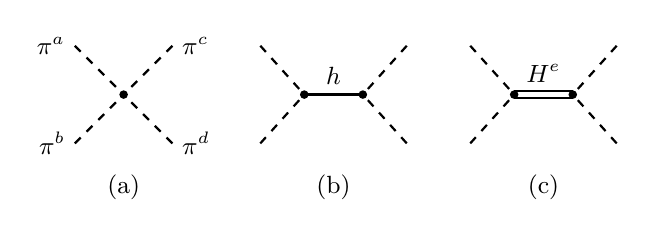
\begin{tikzpicture}[scale=0.62,
  pion/.style={dashed,thick},
  scal/.style={thick},
  heavy/.style={double,double distance=1.6pt,thick}]
% contact
\begin{scope}[shift={(0,0)}]
\draw[pion] (-1,1)--(0,0); \draw[pion] (-1,-1)--(0,0);
\draw[pion] (1,1)--(0,0);  \draw[pion] (1,-1)--(0,0);
\fill (0,0) circle (2.5pt);
\node[left] at (-1,1) {\small $\pi^a$}; \node[left] at (-1,-1) {\small $\pi^b$};
\node[right] at (1,1) {\small $\pi^c$}; \node[right] at (1,-1) {\small $\pi^d$};
\node at (0,-1.9) {\small (a)};
\end{scope}
% h exchange
\begin{scope}[shift={(4.3,0)}]
\draw[pion] (-1.5,1)--(-0.6,0); \draw[pion] (-1.5,-1)--(-0.6,0);
\draw[pion] (1.5,1)--(0.6,0);  \draw[pion] (1.5,-1)--(0.6,0);
\draw[scal] (-0.6,0)--(0.6,0); \fill (-0.6,0) circle (2.5pt); \fill (0.6,0) circle (2.5pt);
\node[above] at (0,0) {\small $h$};
\node at (0,-1.9) {\small (b)};
\end{scope}
% H exchange
\begin{scope}[shift={(8.6,0)}]
\draw[pion] (-1.5,1)--(-0.6,0); \draw[pion] (-1.5,-1)--(-0.6,0);
\draw[pion] (1.5,1)--(0.6,0);  \draw[pion] (1.5,-1)--(0.6,0);
\draw[heavy] (-0.6,0)--(0.6,0); \fill (-0.6,0) circle (2.5pt); \fill (0.6,0) circle (2.5pt);
\node[above] at (0,0.05) {\small $H^e$};
\node at (0,-1.9) {\small (c)};
\end{scope}
\end{tikzpicture}
\caption{Tree-level diagrams for $\pi^a\pi^b\to\pi^c\pi^d$ in the L$\Sigma$M: (a) four-NGB contact interaction of the NL$\Sigma$M, Eq.~\eqref{eq:LNLSM}; (b) exchange of the radial singlet $h$; (c) exchange of the radial multiplet $H^e$. Only the $s$-channel exchange is shown; the $t$- and $u$-channel diagrams are obtained by crossing. Dashed lines: NGBs; solid line: $h$; double line: $H^e$.}
\label{fig:diagrams}
\end{figure}

\subsection{The exact tree-level amplitude}

The amplitude for $\pi^A\pi^B\to\pi^C\pi^D$ receives the contributions of Fig.~\ref{fig:diagrams}. Inserting $g^E_{AB}=d^{ABE}$ in Eq.~\eqref{eq:Arho} and using the identity proven below, the $\mathcal{O}(s)$ terms cancel exactly and we obtain the closed form
\begin{equation}
\begin{split}
\mathcal{A}={}&-\sum_{E=0}^{D}\frac{m_E^2}{f^2}\bigg[d^{ABE}d^{CDE}\frac{s}{s-m_E^2}\\
&+d^{ACE}d^{BDE}\frac{t}{t-m_E^2}+d^{ADE}d^{BCE}\frac{u}{u-m_E^2}\bigg],
\end{split}
\label{eq:Afull}
\end{equation}
with $m_0=m_h$ and $m_{e}=m_H$. Equation~\eqref{eq:Afull} holds for the three families and includes the scattering of $\eta$. At low energy, $s/(s-m^2)\to-s/m^2$ and $\mathcal{A}$ reproduces the NL$\Sigma$M amplitude in the Jordan form
\begin{equation}
\mathcal{A}_{\rm NL\Sigma M}=\frac{s\,d^{ABE}d^{CDE}+t\,d^{ACE}d^{BDE}+u\,d^{ADE}d^{BCE}}{f^2},
\label{eq:ANLSMd}
\end{equation}
equivalent to Eq.~\eqref{eq:ANLSM} by virtue of Eq.~\eqref{eq:identity}. At high energy, $s\gg m_{h,H}^2$, the amplitude approaches a constant,
\begin{equation}
\begin{split}
\mathcal{A}\;\xrightarrow{s\to\infty}\;&-\frac{1}{f^2}\sum_E m_E^2\big(d^{ABE}d^{CDE}+d^{ACE}d^{BDE}\\&+d^{ADE}d^{BCE}\big)+\mathcal{O}\Big(\frac{m^4}{s}\Big),
\end{split}
\label{eq:Ainf}
\end{equation}
of order $m^2/f^2\sim\lambda$, as expected for a renormalizable theory. We have checked Eq.~\eqref{eq:Afull} numerically against the Feynman rules of Eq.~\eqref{eq:expanded}.

The cancellation of the $E^2$ growth rests on the following identity, which is the Gauss equation~\eqref{eq:Gauss} for the minimal completion.

\begin{lemma}
\label{lem:identity}
For the three families, with $f^{ABI}$ and $d^{ABC}$ defined in Eqs.~\eqref{eq:fdef} and~\eqref{eq:ddef},
\begin{equation}
f^{ABI}f^{CDI}=d^{ACE}d^{BDE}-d^{ADE}d^{BCE}.
\label{eq:identity}
\end{equation}
\end{lemma}
\begin{proof}
For any four matrices, expanding the products and using the cyclicity of the trace,
\begin{equation}
\begin{split}
&\Tr\big(\{X^A,X^C\}\{X^B,X^D\}\big)-\Tr\big(\{X^A,X^D\}\{X^B,X^C\}\big)\\
&\qquad=-\Tr\big([X^A,X^B][X^C,X^D]\big).
\end{split}
\label{eq:traceid}
\end{equation}
By Eq.~\eqref{eq:symmetric}, $[X^A,X^B]=if^{ABI}T^I$, and the right-hand side equals $\tfrac12f^{ABI}f^{CDI}$. By the Jordan property~\eqref{eq:ddef}, $\{X^A,X^C\}=d^{ACE}X^E$, and the left-hand side equals $\tfrac12(d^{ACE}d^{BDE}-d^{ADE}d^{BCE})$.
\end{proof}
Separating the singlet $E=0$ and restricting to non-abelian indices, Eq.~\eqref{eq:identity} reads
\begin{equation}
f^{abI}f^{cdI}=\underbrace{\frac{2}{n}\big(\delta^{ac}\delta^{bd}-\delta^{ad}\delta^{bc}\big)}_{h\ \text{exchange}}+\underbrace{d^{ace}d^{bde}-d^{ade}d^{bce}}_{H\ \text{exchange}} ,
\label{eq:identity2}
\end{equation}
which for the chiral coset is the well-known $SU(N)$ relation~\cite{Haber:2019sgz}. The left-hand side is the $E^2$ growth of the NL$\Sigma$M, and the two terms on the right are the contributions of $h$ and of $H^a$ exchange.

The proof is the same for the three families: it uses only the symmetric-space property~\eqref{eq:symmetric} and the Jordan property~\eqref{eq:ddef}. Note that Eq.~\eqref{eq:identity2} cannot be replaced by its isotropic average $f^{abI}f^{cdI}\to\bar K(\delta^{ac}\delta^{bd}-\delta^{ad}\delta^{bc})$, which is exact only for $N=2$ (Proposition~\ref{prop:sphere}).

\subsection{Truncations: which radial modes are necessary}

\emph{$N=2$.} For $N=2$, $d^{abc}=0$ and Eq.~\eqref{eq:identity2} is saturated by $h$ alone, with coupling $g_h^2=2/n=\bar K$. In the $\pi^a$ sector the multiplet $H^a$ decouples, and one recovers the $O(4)$, $O(3)$ and $O(6)$ models. In the SM case the result is the familiar statement that the Higgs boson, with SM couplings, unitarizes $W_LW_L$ scattering~\cite{Lee:1977eg}. If the $U(1)$ NGB $\eta$ is kept, $H^a$ is still needed. The NL$\Sigma$M amplitude for $\pi^a\eta\to\pi^b\eta$ vanishes, since $f^{a0I}=0$, but the $t$-channel exchange of $h$ grows as $-(2/n)\,t\,\delta^{ab}/f^2$. It is cancelled by the $s$- and $u$-channel exchange of $H^a$, through $d^{a0e}d^{b0e}=\frac{2}{n}\delta^{ab}$, which is Eq.~\eqref{eq:identity} with $B=D=0$. As discussed in Sec.~\ref{sec:beyond}, this extra multiplet can be avoided by using a smaller \emph{reducible} representation.

\emph{$N\geq3$.} Dropping $H^a$ leaves in $\pi\pi\to\pi\pi$ the residual growth $f^{-2}\big[s\,d^{abe}d^{cde}+t\,d^{ace}d^{bde}+u\,d^{ade}d^{bce}\big]$, which does not vanish because, by Proposition~\ref{prop:sphere}, the right-hand side of Eq.~\eqref{eq:identity2} cannot be proportional to $\delta\delta-\delta\delta$. Dropping $h$ leaves a residual growth proportional to $\frac2n(\delta^{ac}\delta^{bd}-\delta^{ad}\delta^{bc})$, which is excluded by Proposition~\ref{prop:singlet}. Since $h$ and $H^a$ are irreducible under $\Hg$, no $\Hg$-invariant partial truncation is possible. Hence:

\begin{proposition}
\label{prop:minimal}
For $N\geq3$, in the minimal linear completion of each of the cosets~\eqref{eq:cosets}, every radial mode (the singlet $h$ and the whole multiplet $H^a$) is necessary to cancel the $\mathcal{O}(E^2)$ growth of $\pi\pi\to\pi\pi$.
\end{proposition}

We confirmed Proposition~\ref{prop:minimal} numerically for $N=3,4$ in the three families: with all radial modes the residual of Eq.~\eqref{eq:Gauss} vanishes to machine precision, while dropping $H^a$ leaves a residual of order one (e.g.\ $2/3$, $2/3$ and $1/3$ in units of $f^{-2}$ for the largest tensor component at $N=3$).

\subsection{Other channels}

\begin{table*}[t]
\caption{Two-to-two processes with NGBs in the external states, and the exchanges that cancel the $\mathcal{O}(E^2)$ terms. In the processes with radial modes in the external states the growth of individual diagrams cancels between contact terms and NGB exchange. ``---'' means that no growth is present diagram by diagram.}
\label{tab:processes}
\begin{ruledtabular}
\begin{tabular}{lcc}
Process & NL$\Sigma$M growth & cancelled by \\
\hline
$\pi\pi\to\pi\pi$ & $s/f^2$ & $h$ ($s,t,u$) and $H$ ($s,t,u$) \\
$\pi\eta\to\pi\eta$ & none & $h$ ($t$) against $H$ ($s,u$) \\
$\pi\pi\to\eta\eta$ & none & $h$ ($s$) against $H$ ($t,u$) \\
$\eta\eta\to\eta\eta$ & none & $h$ exchanges add up to $s+t+u=0$ \\
$\pi\pi\to hh$, $\pi\pi\to HH$, $\pi\pi\to hH$ & --- & contact against $\pi$ exchange \\
$\pi h\to\pi h$, $\pi H\to\pi H$, $\pi h\to\pi H$ & --- & crossing of the above
\end{tabular}
\end{ruledtabular}
\end{table*}

Equation~\eqref{eq:Afull} covers all processes with four NGBs, including $\eta$. Table~\ref{tab:processes} summarizes how the cancellations work. For example, in $\pi^a\pi^b\to\eta\eta$ the $s$-channel $h$ exchange and the $t$, $u$-channel $H$ exchange give $\frac2n(s+t+u)\delta^{ab}=0$. In processes with external radial modes, such as $\pi\pi\to hh$, the growth of the $\rho\rho\partial\pi\partial\pi$ contact terms cancels against the $t$- and $u$-channel NGB exchange, leaving terms of order $m^2/f^2$. That only $h$ is required in some channels does not contradict Proposition~\ref{prop:minimal}: a single channel requiring $H^a$ suffices.

%=====================================================================
\section{Beyond the minimal representation}
\label{sec:beyond}
%=====================================================================

The minimal completion is not the only one: larger representations containing the same orbit also give renormalizable, unitary theories. The Gauss equation~\eqref{eq:Gauss} allows us to ask which radial content is compulsory in \emph{any} completion. By $\Hg$-invariance, a radial multiplet in an irreducible representation $R$ of $\Hg$ couples to $\pi^a\pi^b$ only if $R\subset{\rm Sym}^2(R_\pi)$, through the corresponding Clebsch--Gordan coefficients. If ${\rm Sym}^2(R_\pi)=\bigoplus_RR$ is multiplicity free, Eq.~\eqref{eq:Gauss} becomes
\begin{equation}
f^{abI}f^{cdI}=\sum_{R}c_R\,\mathcal{T}_R^{abcd},\qquad c_R\ge0,
\label{eq:GaussR}
\end{equation}
where $\mathcal{T}_R^{abcd}=P_R^{(ac)(bd)}-P_R^{(ad)(bc)}$, $P_R$ is the projector onto $R$ in ${\rm Sym}^2(R_\pi)$, and $c_R$ is the sum of the squared couplings of all the radial multiplets transforming as $R$. Since $\sum_RP_R$ is the identity on ${\rm Sym}^2$, one has $\sum_R\mathcal{T}_R=-\frac{D}{2}\mathcal{T}_{\bf 1}$ identically.

\begin{proposition}[rigidity for $N=3$]
\label{prop:rigidity}
For $N=3$, ${\rm Sym}^2(R_\pi)={\bf 1}\oplus R_\pi\oplus R_3$, namely ${\bf 1}\oplus{\bf 8}\oplus{\bf 27}$ of $SU(3)$, ${\bf 1}\oplus{\bf 5}\oplus{\bf 9}$ of $SO(3)$, and ${\bf 1}\oplus{\bf 14}\oplus{\bf 90}$ of $Sp(6)$. Every linear completion contains a radial singlet and a radial multiplet in $R_\pi$, with
\begin{equation}
c_{\bf 1}\ge c_{\bf 1}^{\rm min},\qquad c_{R_\pi}\ge c_{R_\pi}^{\rm min},
\label{eq:rigidity}
\end{equation}
where the superscript denotes the values of the minimal completion of Sec.~\ref{sec:LSM}. Equality holds if and only if no radial modes in $R_3$ couple to the NGBs.
\end{proposition}
\begin{proof}
The three tensors $\mathcal{T}_R$ span a two-dimensional space: $\mathcal{T}_{\bf 1}\propto\delta\delta-\delta\delta$ and $\mathcal{T}_{R_\pi}$ are independent (the latter has a component along $f^{abI}f^{cdI}$), and they obey the relation $(1+\frac D2)\mathcal{T}_{\bf 1}+\mathcal{T}_{R_\pi}+\mathcal{T}_{R_3}=0$. We have checked explicitly that it is the only one. Subtracting the minimal solution, which has $c_{R_3}=0$, from a generic solution of Eq.~\eqref{eq:GaussR} gives $(c_{\bf 1}-c^{\rm min}_{\bf 1},\,c_{R_\pi}-c^{\rm min}_{R_\pi},\,c_{R_3})=\kappa\,(1+\tfrac D2,1,1)$, and positivity of $c_{R_3}$ requires $\kappa\ge0$.
\end{proof}

In physical terms, for $N=3$ the radial multiplet in $R_\pi$ cannot be traded for a multiplet in another representation: adding radial modes in $R_3$ \emph{increases} the required couplings of $h$ and $H$. In terms of couplings, Eq.~\eqref{eq:rigidity} reads $\sum g_{h_r}^2\ge 2/n$ for the singlets and $\sum\kappa_r^2\ge1$ for multiplets coupling as $\kappa_r d^{abc}$.

For $N\ge4$, ${\rm Sym}^2(R_\pi)$ contains four irreducible components: ${\bf 1}\oplus{\bf 15}\oplus{\bf 20}'\oplus{\bf 84}$ for $SU(4)$, ${\bf 1}\oplus{\bf 9}\oplus{\bf 10}\oplus{\bf 25}$ for $SO(4)$, and ${\bf 1}\oplus{\bf 27}\oplus{\bf 42}\oplus{\bf 308}$ for $Sp(8)$. We find that the tensors $\mathcal{T}_R$ still span the two-dimensional space generated by $\delta\delta-\delta\delta$ and $f^{abI}f^{cdI}$, but now a second non-singlet representation ($R'={\bf 20}'$, ${\bf 10}$, ${\bf 42}$) has a positive component along $f^{abI}f^{cdI}$. Writing $\mathcal{T}_R=\alpha_R(\delta\delta-\delta\delta)+\beta_R\,ff$, we find $\beta_{R'}>0$ and $\alpha_{R'}<0$ (e.g.\ $\mathcal{T}_{{\bf 20}'}=-\frac16(\delta\delta-\delta\delta)+\frac14ff$ for $SU(4)$). The Gauss equation alone therefore allows, in principle, completions in which the role of $H^a$ is played by radial modes in $R'$. Whether such completions are realized by representations of $\G$ with the required vacuum is a question that the sum rules cannot answer, and that we leave for future work. Propositions~\ref{prop:singlet} and~\ref{prop:sphere} hold for all $N$.

A different loophole concerns the $U(1)$ sector. For $N=2$, the $U(1)$-extended chiral coset is $S^3\times S^1$ (up to a discrete quotient), which can be completed by the reducible representation $({\bf 2},{\bf 2})_{\mathbb R}\oplus{\bf 1}_{\mathbb C}$ with six real fields, instead of the eight of $({\bf 2},{\bf 2})_{\mathbb C}$. Here $\eta$ is the phase of a separate complex singlet and the triplet $H^a$ is not needed. This illustrates the point raised above: a minimal \emph{irreducible} representation need not be the minimal completion when $\G$ has several factors. For $N\ge3$ and for the non-abelian NGBs, Propositions~\ref{prop:minimal} and~\ref{prop:rigidity} show that this does not happen.

%=====================================================================
\section{Perturbative unitarity and the mass scale of the radial modes}
\label{sec:unitarity}
%=====================================================================

\begin{table*}[t]
\caption{Eigenvalues $e$ of the $s$-wave scattering matrix at high energy, $a_0=-e/(16\pi)$, in units of the couplings of Eq.~\eqref{eq:V}, and their multiplicities (number of real two-particle states). States are classified by $SU(N)_L\times SU(N)_R$ (chiral coset), by $SU(N)$ (second family) and by $SU(2N)$ (third family), and by whether they are built out of $\Hf\Hf$ (and conjugate) or $\Hf\Hf^\dagger$.}
\label{tab:unitarity}
\begin{ruledtabular}
\begin{tabular}{llc}
Channel & $e$ & multiplicity \\
\hline
\multicolumn{3}{l}{$SU(N)\times SU(N)/SU(N)$, $D_{\mathbb R}=2N^2$}\\
$\Hf\Hf^\dagger$, $({\bf 1},{\bf 1})$ & $(2N^2+2)\lambda_1+4N\lambda_2$ & $1$\\
$\Hf\Hf^\dagger$, $({\rm adj},{\bf 1})\oplus({\bf 1},{\rm adj})$ & $2\lambda_1+2N\lambda_2$ & $2(N^2-1)$\\
$\Hf\Hf^\dagger$, $({\rm adj},{\rm adj})$ & $2\lambda_1$ & $(N^2-1)^2$\\
$\Hf\Hf$, $(S,S)$ & $2\lambda_1+2\lambda_2$ & $N^2(N+1)^2/2$\\
$\Hf\Hf$, $(A,A)$ & $2\lambda_1-2\lambda_2$ & $N^2(N-1)^2/2$\\
\hline
\multicolumn{3}{l}{$SU(N)/SO(N)$, $D_{\mathbb R}=N(N+1)$}\\
$\Hf\Hf^\dagger$, singlet & $(N^2+N+2)\lambda_1+2(N+1)\lambda_2$ & $1$\\
$\Hf\Hf^\dagger$, adjoint & $2\lambda_1+(N+2)\lambda_2$ & $N^2-1$\\
$\Hf\Hf^\dagger$, other & $2\lambda_1$ & $N^2(N-1)(N+3)/4$\\
$\Hf\Hf$, $[4]$ & $2\lambda_1+2\lambda_2$ & $N(N+1)(N+2)(N+3)/12$\\
$\Hf\Hf$, $[2,2]$ & $2\lambda_1-\lambda_2$ & $N^2(N^2-1)/6$\\
\hline
\multicolumn{3}{l}{$SU(2N)/Sp(2N)$, $D_{\mathbb R}=2N(2N-1)$, $M\equiv2N$}\\
$\Hf\Hf^\dagger$, singlet & $(M^2-M+2)\lambda_1+2(M-1)\lambda_2$ & $1$\\
$\Hf\Hf^\dagger$, adjoint & $2\lambda_1+(M-2)\lambda_2$ & $M^2-1$\\
$\Hf\Hf^\dagger$, other & $2\lambda_1$ & $M^2(M+1)(M-3)/4$\\
$\Hf\Hf$, $[2,2]$ & $2\lambda_1+\lambda_2$ & $M^2(M^2-1)/6$\\
$\Hf\Hf$, $[1^4]$ & $2\lambda_1-2\lambda_2$ & $M(M-1)(M-2)(M-3)/12$
\end{tabular}
\end{ruledtabular}
\end{table*}

\begin{figure}[t]
\centering
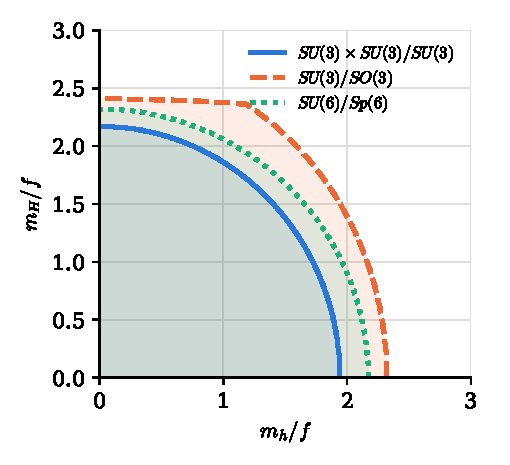
\includegraphics[width=0.95\columnwidth]{../figures/unitarity_N3.pdf}
\caption{Region of the $(m_h/f,\,m_H/f)$ plane allowed by tree-level perturbative unitarity, $|{\rm Re}\,a_0|\le\frac12$ in all the channels of Table~\ref{tab:unitarity}, for $N=3$: $SU(3)\times SU(3)/SU(3)$ (solid), $SU(3)/SO(3)$ (dashed) and $SU(6)/Sp(6)$ (dotted). The allowed region lies below each curve.}
\label{fig:unitarity}
\end{figure}

The L$\Sigma$M is weakly coupled as long as the quartic couplings, \ie\ $m_{h,H}^2/f^2$, are perturbative. At energies $E\gg m_{h,H}$ all two-to-two amplitudes among the $D_{\mathbb R}$ real components of $\Hf$ approach their contact values, $\mathcal{A}_{ij\to kl}=-\partial^4V/\partial\phi_i\partial\phi_j\partial\phi_k\partial\phi_l$, and the $s$-wave amplitudes are $a_0=-e/(16\pi)$, where $e$ are the eigenvalues of the quartic-coupling matrix on the two-particle states (including the factor $1/\sqrt2$ for identical particles). Decomposing the two-particle states into irreducible representations of $\G$, we obtain the eigenvalues of Table~\ref{tab:unitarity}, which we have also computed numerically for $N\le4$. Imposing $|{\rm Re}\,a_0|\le\frac12$ and using Eq.~\eqref{eq:masses}, the singlet channel, which is the most constraining one for $\lambda_1\ge0$, gives
\begin{equation}
(D_{\mathbb R}+2)\,m_h^2+(D_{\mathbb R}-2)\,m_H^2\;\le\;8\pi\,n\,f^2 .
\label{eq:unitarity_singlet}
\end{equation}
For degenerate radial modes, $m_h=m_H\equiv m$, the bound reads
\begin{equation}
m\le\sqrt{\frac{2\pi}{N}}\,f,\qquad m\le\sqrt{\frac{4\pi}{N+1}}\,f,\qquad m\le\sqrt{\frac{4\pi}{2N-1}}\,f
\label{eq:unitarity_deg}
\end{equation}
for the three families. As a check, for the $O(4)$ model with $f=v=246$~GeV the same procedure gives the classic bound $m_h\lesssim710$~GeV~\cite{Lee:1977eg}. The allowed region for $N=3$, including all channels, is shown in Fig.~\ref{fig:unitarity}. The radial modes of a weakly coupled completion must therefore lie at or below $\sim(1$--$2)\,f$, with the window shrinking as $1/\sqrt N$ at large $N$: the larger the coset, the lighter the radial modes must be for the linear completion to remain perturbative.

%=====================================================================
\section{Phenomenological remarks}
\label{sec:pheno}
%=====================================================================

The analysis above is model independent, but it has direct implications when the NL$\Sigma$M describes electroweak symmetry breaking. We discuss three aspects.

\emph{Higgs couplings and sum rules.} If the electroweak group is gauged inside $\G$, three NGBs are eaten by $W^\pm$ and $Z$. By the equivalence theorem, the projection of Eq.~\eqref{eq:Gauss} onto the eaten directions is the sum rule $\sum_r\kappa_{V,r}^2=1$, where $\kappa_{V,r}$ is the coupling of the radial mode $r$ to $VV$ in units of the SM Higgs coupling~\cite{Gunion:1990kf,Falkowski:2012vh}. For $N=2$ the radial singlet has exactly the SM couplings, and the SM Higgs sector is the $N=2$ chiral L$\Sigma$M; the $SU(4)/Sp(4)$ case reproduces the elementary Goldstone Higgs models of Refs.~\cite{Alanne:2014kea,Gertov:2015xma,Cacciapaglia:2014uja}. For $N\ge3$ the distribution of the sum rule among $h$ and $H$ depends on how $SU(2)_L\times U(1)_Y$ is embedded, \ie\ on vacuum alignment~\cite{Peskin:1980gc,Preskill:1980mz}. If $SU(2)_L$ acts on $N/2$ copies of a doublet, as in one-family technicolor, the eaten generators satisfy $\{t^a,t^b\}\propto\delta^{ab}\mathbb{1}$ and only $h$ couples to $W_LW_L$, with $\kappa_V=1$. If instead $SU(2)_L$ acts on a single $2\times2$ block, $h$ and the custodial-singlet component of $H$ share the sum rule, $\kappa_V^2(h)=2/n$ and $\kappa_V^2(H)=1-2/n$. The LHC measurements of the Higgs couplings to weak bosons, consistent with the SM at the level of several percent~\cite{ATLAS:2022vkf,CMS:2022dwd,ParticleDataGroup:2024cfk}, require the $125$~GeV state to saturate the sum rule. In the second embedding this excludes the identification of the observed Higgs with a pure radial singlet, and predicts additional scalar resonances coupled to $W_LW_L$, a target for searches of heavy resonances decaying to $VV$.

\emph{Mass scale of the radial modes.} The masses $m_h^2=(n\lambda_1+\lambda_2)f^2$ and $m_H^2=\lambda_2f^2$ are free parameters of the L$\Sigma$M, bounded from above by Eqs.~\eqref{eq:unitarity_singlet} and~\eqref{eq:unitarity_deg}. In composite Higgs scenarios, where the Higgs is itself one of the NGBs and $\xi=v^2/f^2\lesssim0.1$ from Higgs coupling measurements and electroweak precision tests~\cite{Peskin:1991sw,ParticleDataGroup:2024cfk,Contino:2010rs,Panico:2015jxa}, this places the radial modes in the TeV range. In technicolor-like embeddings with $f\simeq v$ and $N\geq3$, the uneaten pseudo-NGBs and the adjoint radial modes are additionally constrained by direct searches and by the $S$ parameter~\cite{Peskin:1991sw}.

\emph{Vacuum stability.} In the SM the running Higgs quartic coupling turns negative at $\Lambda_I\sim10^{10}$--$10^{11}$~GeV for the central value of the top mass, and the electroweak vacuum is metastable. The conclusion depends crucially on $m_t$: absolute stability would require $m_t\lesssim171$~GeV~\cite{Sher:1988mj,Degrassi:2012ry,Buttazzo:2013uya}. Additional weakly coupled scalars contribute positively to the beta function of the Higgs quartic and can stabilize the potential, in particular through tree-level threshold effects when they mix with the Higgs~\cite{Elias-Miro:2012eoi,Lebedev:2012zw}. The radial modes of an L$\Sigma$M completion are natural candidates for this mechanism, provided they lie below $\Lambda_I$. A quantitative analysis requires specifying how the SM Higgs and the top quark are embedded, and is beyond the scope of this work.

%=====================================================================
\section{Further results}
\label{sec:further}
% =====================================================================
%  New material for "Higgs radial modes in linear completions of NLSMs"
%  Four self-contained subsections, ready to be inserted in the paper.
%  Notation follows the paper: X^A (A=0..D) broken generators with X^0 = 1/sqrt(2n),
%  d^{ABC} Jordan symbols, f^{abI}f^{cdI} = F^{abcd}, A^{abcd} = d^{ac}d^{bd} - d^{ad}d^{bc}.
%  Numerical checks: checks/p1_lecs.py, p2_realize.py, p4_octonion.py.
%  Bibliography keys: refs.bib + additions/additions.bib.
% =====================================================================

% ---------------------------------------------------------------------
\subsection{Low-energy constants and positivity}
\label{add:lecs}
% ---------------------------------------------------------------------

Integrating out the radial modes at tree level determines the four-derivative chiral Lagrangian. In the closed-form Lagrangian~\eqref{eq:master} the radial modes couple linearly to the NGBs through $\frac14\Tr\{d_\mu,\Phi\}^2\supset 2f\,\Tr(\hat\rho\, d_\mu d^\mu)$, with $\hat\rho=2\rho^CX^C$. The source of $\rho^C$ is therefore $J^C=4f\,\Tr(X^C d_\mu d^\mu)$, which at lowest order reproduces the cubic couplings $\frac1f d^{ABC}\rho^C\partial\pi^A\!\cdot\partial\pi^B$. Since $d_\mu d^\mu=\frac12\{d_\mu,d^\mu\}$ belongs to the Jordan algebra, the completeness of the basis $X^C$ gives, for the three families,
\begin{equation}
\begin{split}
\mathcal L_4={}&\frac{4f^2}{n\,m_h^2}\big[\Tr(d_\mu d^\mu)\big]^2\\
&+\frac{4f^2}{m_H^2}\Big\{\Tr\big(d_\mu d^\mu d_\nu d^\nu\big)-\frac1n\big[\Tr(d_\mu d^\mu)\big]^2\Big\}+\mathcal O(p^6).
\end{split}
\label{eq:L4tree}
\end{equation}
In the basis $\langle u_\mu u^\mu\rangle^2$, $\langle u_\mu u_\nu\rangle\langle u^\mu u^\nu\rangle$, $\langle u_\mu u^\mu u_\nu u^\nu\rangle$, $\langle u_\mu u_\nu u^\mu u^\nu\rangle$, with $u_\mu=2d_\mu$ and leading-order Lagrangian $\frac{f^2}{4}\langle u_\mu u^\mu\rangle$, Eq.~\eqref{eq:L4tree} corresponds to
\begin{equation}
\begin{split}
&L_1=\frac{f^2}{4n}\Big(\frac{1}{m_h^2}-\frac{1}{m_H^2}\Big),\qquad L_3=\frac{f^2}{4m_H^2},\\
&L_0=L_2=0 ,
\end{split}
\label{eq:LECs}
\end{equation}
where $n$ is the size of the matrices. For specific $N$ the Cayley--Hamilton relations reduce the operator basis~\cite{Bijnens:2009qm,Bijnens:2011fm}. Equation~\eqref{eq:LECs} is the linear-sigma-model counterpart of resonance saturation~\cite{Ecker:1988te}. For $n=3$, the radial octet gives $L_1=-L_3/3$ and $L_3=c_d^2/(2m_H^2)$ with $c_d=f/\sqrt2$. The radial singlet gives $L_1=\tilde c_d^{\,2}/(2m_h^2)$ with $\tilde c_d=c_d/\sqrt3$, which is the nonet relation. As for scalar resonances in QCD, $L_0$ and $L_2$ are not generated at this order.

The same coefficients follow from the low-energy expansion of the exact amplitude~\eqref{eq:Afull}:
\begin{equation}
\begin{split}
\mathcal A^{(4)}=\frac{1}{f^2}\sum_{E=0}^{D}\frac{1}{m_E^2}\Big[&d^{ABE}d^{CDE}s^2+d^{ACE}d^{BDE}t^2\\
&+d^{ADE}d^{BCE}u^2\Big].
\end{split}
\label{eq:A4}
\end{equation}
We have checked numerically that the Feynman rules of Eq.~\eqref{eq:L4tree} reproduce Eq.~\eqref{eq:A4}, including $\eta$, for the three families. Equation~\eqref{eq:A4} makes the positivity of the completion manifest. For arbitrary real superpositions $|\alpha\rangle=\alpha^A\pi^A$ and $|\beta\rangle=\beta^B\pi^B$, the forward elastic amplitude has
\begin{equation}
\begin{split}
&\frac{1}{2}\frac{\partial^2}{\partial s^2}\mathcal A(\alpha\beta\to\alpha\beta)\Big|_{t=0}\\
&\qquad=\frac{2}{f^2}\sum_E\frac{(\alpha^Ad^{ABE}\beta^B)^2}{m_E^2}\;\ge\;0 .
\end{split}
\end{equation}
The radial modes therefore satisfy, flavor by flavor, the positivity bounds that analyticity and unitarity impose on the $\mathcal O(p^4)$ coefficients~\cite{Adams:2006sv,Manohar:2008tc}. The bounds are saturated by contributions of the form ``coupling squared over mass squared'', and the Gauss equation fixes the corresponding $\mathcal O(p^2)$ sum rule.

% ---------------------------------------------------------------------
\subsection{Non-minimal completions at $N=4$ are realized}
\label{add:N4}
% ---------------------------------------------------------------------

The Gauss equation allows, for $N\ge4$, solutions in which the radial multiplet with the NGB quantum numbers is replaced by a second irreducible representation $R'$ of $\Hg$ in ${\rm Sym}^2(R_\pi)$: $\mathbf{20}'$ for $SU(4)$, $\mathbf 5_L\oplus\mathbf 5_R$ for $SO(4)$, and $\mathbf{42}$ for $Sp(8)$. We now show that these solutions are realized by explicit linear representations of $\G$. For a field in a representation with generators $t_\alpha$ and vacuum $v$, we compute three quantities directly from the representation: the intrinsic curvature of the orbit, $F^{abcd}=-(t_cv)\cdot([[t_a,t_b],t_d]v)/f^2$; the second fundamental form, Eq.~\eqref{eq:cubicgeneric}; and the decomposition of the normal couplings into irreducible representations of $\Hg$.

\begin{enumerate}
\item \emph{$SU(4)\times SU(4)/SU(4)$ via a real $(\mathbf6,\mathbf6)$.} Since $SU(4)\simeq Spin(6)$, the antisymmetric $\mathbf6=\Lambda^2\mathbf4$ is real. A real $6\times6$ matrix field $\mathcal O\to L_6\,\mathcal O\,R_6^T$ with $\langle\mathcal O\rangle\propto\mathbb{1}$ breaks $SU(4)_L\times SU(4)_R$ to $SU(4)_V$. The 36 real fields contain the 15 NGBs in the antisymmetric part and the radial modes in the symmetric part, ${\rm Sym}^2\mathbf6=\mathbf1\oplus\mathbf{20}'$. No radial adjoint exists. The potential $V=-\frac{\mu^2}{2}\Tr\mathcal O\mathcal O^T+\frac{\lambda_1}{4}(\Tr\mathcal O\mathcal O^T)^2+\frac{\lambda_2}{4}\Tr(\mathcal O\mathcal O^T)^2$ with $\lambda_2>0$ has its minimum along $\mathbb{1}$, as in Sec.~\ref{sec:LSM}.
\item \emph{$SU(4)/SO(4)$ via the $\mathbf{20}'$.} With $SU(4)/SO(4)\simeq SO(6)/SO(3)\times SO(3)$, a real symmetric traceless $6\times6$ matrix $S\to OSO^T$ with $\langle S\rangle\propto{\rm diag}(1,1,1,-1,-1,-1)$ has stabilizer $SO(3)\times SO(3)\simeq SO(4)$. Of its 20 components, 9 are NGBs and the radial modes are $\mathbf1\oplus\mathbf5_L\oplus\mathbf5_R$. For a potential even in $S$ with positive coefficient of $\Tr S^4$, this vacuum is the minimum: at fixed $\Tr S^2$, $\Tr S^4$ is minimal when all six eigenvalues have equal modulus.
\item \emph{$SU(8)/Sp(8)$ via $\Lambda^4\mathbf8$.} The four-form representation of $SU(8)$ is real ($\mathbf{70}$). The vacuum $\omega\wedge\omega$, with $\omega$ the symplectic form, has stabilizer $Sp(8)$. Under $Sp(8)$, $\mathbf{70}=\mathbf1\oplus\mathbf{27}\oplus\mathbf{42}$: the $\mathbf{27}$ are the NGBs and the radial modes are $\mathbf1\oplus\mathbf{42}$. Since the $Sp(8)$-invariant subspace is one dimensional, this orbit is critical for every $SU(8)$-invariant potential at the radius that minimizes the potential along the invariant direction~\cite{Michel:1971}. Whether it is a minimum depends on the quartic couplings, and we do not analyze it further.
\end{enumerate}

\begin{table*}[t]
\caption{Share of the curvature term $f^{abI}f^{cdI}$ in the Gauss equation carried by each radial multiplet coupled to $\pi\pi$, for several linear completions. In all cases the residual of the Gauss equation vanishes to machine precision ($\lesssim5\times10^{-16}$). The singlet only contributes to $\delta\delta-\delta\delta$ and is not listed.}
\label{tab:shares}
\begin{ruledtabular}
\begin{tabular}{llll}
coset & field & radial multiplets coupled to $\pi\pi$ & share of $f^{abI}f^{cdI}$\\
\hline
$SU(3)^2/SU(3)$ & $(\mathbf3,\bar{\mathbf3})$ (minimal) & $\mathbf1,\ \mathbf8$ & $\mathbf8$: $1$\\
$SU(3)^2/SU(3)$ & $(\mathbf8,\mathbf8)$ & $\mathbf1,\ \mathbf8,\ \mathbf{27}$ & $\mathbf8$: $9/5$;\ \ $\mathbf{27}$: $-4/5$\\
$SU(4)^2/SU(4)$ & $(\mathbf6,\mathbf6)_{\mathbb R}$ & $\mathbf1,\ \mathbf{20}'$ & $\mathbf{20}'$: $1$\\
$SU(4)/SO(4)$ & $\mathbf{20}'$ of $SO(6)$ & $\mathbf1,\ \mathbf5_L\oplus\mathbf5_R$ & $\mathbf5_L\oplus\mathbf5_R$: $1$\\
$SU(8)/Sp(8)$ & $\Lambda^4\mathbf8=\mathbf{70}$ & $\mathbf1,\ \mathbf{42}$ & $\mathbf{42}$: $1$\\
$SU(5)^2/SU(5)$ & $(\mathbf{10},\overline{\mathbf{10}})$ & $\mathbf1,\ \mathbf{24},\ \mathbf{75}$ & $\mathbf{24}$: $1/9$;\ \ $\mathbf{75}$: $8/9$
\end{tabular}
\end{ruledtabular}
\end{table*}

The results are collected in Table~\ref{tab:shares}. The $(\mathbf8,\mathbf8)$ completion of $SU(3)\times SU(3)/SU(3)$ illustrates Proposition~\ref{prop:rigidity}: the radial $\mathbf{27}$ contributes with negative sign, and the octet coupling is correspondingly larger than in the minimal model. In the three $N=4$ completions the multiplet with the NGB quantum numbers is absent, and the curvature is carried entirely by $R'$. Rigidity is therefore sharp: it holds at $N=3$ and fails at $N=4$ in all three families.

The mechanism is transparent in the chiral case. For a field in $(R,\bar R)$, the coupling of a radial adjoint to $\pi\pi$ is proportional to the symmetric trace $\Tr_R(\{T^a,T^b\}T^c)=A(R)\,d^{abc}/2$, i.e.\ to the anomaly coefficient of $R$. For $R=\Lambda^2\mathbf N$, $A(R)=N-4$: it vanishes at $N=4$, where $\Lambda^2\mathbf4$ is real, and it is small at $N=5$. This is reflected in the small share $1/9$ of the $\mathbf{24}$ in the $(\mathbf{10},\overline{\mathbf{10}})$ completion. The $N=4$ examples also show that completions with the same number of fields can differ in their radial content. For $SU(4)/SO(4)$, both the complex two-index symmetric $\mathbf{10}$ and the real $\mathbf{20}'$ have 20 real components, with radial modes $\mathbf1\oplus\mathbf9$ and $\mathbf1\oplus\mathbf5_L\oplus\mathbf5_R$ respectively (the former also contains the $U(1)$ NGB). The minimal irreducible representation is not unique.

% ---------------------------------------------------------------------
\subsection{QCD and lattice spectra}
\label{add:qcd}
% ---------------------------------------------------------------------

The unitarity bounds of Sec.~\ref{sec:unitarity} give a quantitative measure of how far a strongly coupled spectrum is from a perturbative linear completion. In QCD with three light flavors, $f\simeq F_\pi\simeq92$~MeV in our normalization. For degenerate radial modes, Eq.~\eqref{eq:unitarity_deg} gives $m\lesssim\sqrt{2\pi/3}\,f\simeq130$~MeV. For the physical scalar spectrum, with $f_0(500)$ at $\sqrt s\simeq(450-i\,275)$~MeV~\cite{Pelaez:2015qba,ParticleDataGroup:2024cfk} and the nonet partner $a_0(980)$, the left-hand side of the singlet-channel condition~\eqref{eq:unitarity_singlet} exceeds the right-hand side by a factor of about~30. Thus the scalar mesons of QCD lie far outside the perturbative window. A linear sigma model reproduces them only with quartic couplings of order $m^2/f^2\sim25$--$100$, consistent with the large width of the $f_0(500)$.

The same conclusion holds for the minimal fundamental composite-Higgs template, $SU(2)$ gauge theory with two fundamental Dirac flavors, i.e.\ the coset $SU(4)/Sp(4)$. Lattice simulations give $m_\sigma/F_{\rm PS}=19(11)$ and $m_{a_0}/F_{\rm PS}=17(5)$~\cite{Arthur:2016ozw}; recent determinations of the singlet are in Ref.~\cite{Bowes:2025sigma}. The bound for $N=2$ in the antisymmetric family is $m\lesssim\sqrt{4\pi/3}\,f\simeq2f$. The lattice values therefore exceed it by about an order of magnitude in mass, independently of factors of $\sqrt2$ between conventions for the decay constant. A weakly coupled linear completion of a composite Higgs sector is thus an additional dynamical assumption rather than an approximation to the known strongly coupled dynamics. This is consistent with the radial modes in the matrix benchmarks of Sec.~\ref{sec:pheno} lying near $f$ rather than near $4\pi f$.

% ---------------------------------------------------------------------
\subsection{The exceptional member: $E_6/F_4$}
\label{add:e6}
% ---------------------------------------------------------------------

Lemma~\ref{lem:identity} is a statement about Jordan algebras and does not require associativity of the underlying matrices. Let $J$ be a Euclidean Jordan algebra with product $x\circ y$, associative trace form $\langle x\circ y,z\rangle=\langle x,y\circ z\rangle$, and multiplication operators $L_x y=x\circ y$. Choose an orthonormal basis with $\langle X^A,X^B\rangle=\frac12\delta^{AB}$ and define
\[
d^{ABC}=4\langle X^A\circ X^B,X^C\rangle,
\]
\[
F^{ABCD}=-8\,\big\langle[L_{X^A},L_{X^B}]X^C,X^D\big\rangle .
\]
Associativity of the trace form gives $\langle X^A\circ(X^B\circ X^C),X^D\rangle=\langle X^B\circ X^C,X^A\circ X^D\rangle$, and hence
\begin{equation}
F^{ABCD}=d^{ACE}d^{BDE}-d^{ADE}d^{BCE}
\label{eq:jordanlemma}
\end{equation}
in two lines. For Hermitian matrices $[L_X,L_Y]Z=\frac14[[X,Y],Z]$, and Eq.~\eqref{eq:jordanlemma} reduces to Eq.~\eqref{eq:identity}. In general, $[L_X,L_Y]$ is a derivation of $J$. The Lie algebra ${\rm Der}(J)\oplus i\,L(J_0)$ is the compact form of the reduced structure algebra, and $F^{ABCD}$ is the curvature of the corresponding symmetric space~\cite{FarautKoranyi}.

By the Jordan--von Neumann--Wigner classification~\cite{Jordan:1933vh}, the simple Euclidean Jordan algebras are $J_N(\mathbb R)$, $J_N(\mathbb C)$, $J_N(\mathbb{H})$, the spin factors, and the exceptional algebra $J_3(\mathbb O)$ of $3\times3$ octonionic Hermitian matrices~\cite{Baez:2001dm}. The spin factors give the spheres, i.e.\ the $O(n)$ models with a single radial singlet. The exceptional algebra gives the symmetric space $E_6/F_4$, with $\dim E_6-\dim F_4=78-52=26$ NGBs. Its minimal linear completion is the complex $\mathbf{27}$ of $E_6$, extended by a $U(1)$ factor, with vacuum along the identity of $J_3(\mathbb O)$. The radial modes are a singlet and a $\mathbf{26}$ of $F_4$, and their couplings to the NGBs are the octonionic Jordan symbols $d^{ABC}$. Together with $SU(3)/SO(3)$, $SU(3)\times SU(3)/SU(3)$ and $SU(6)/Sp(6)$, $E_6/F_4$ completes the $J_3(\mathbb K)$ row of the Freudenthal--Tits magic square~\cite{Freudenthal:1964,Tits:1966,GurseyTze}.

The rigidity argument of Sec.~\ref{sec:beyond} applies unchanged. The rank of $E_6/F_4$ is two, so $f^{abI}f^{cdI}$ and $\delta\delta-\delta\delta$ are independent. Moreover ${\rm Sym}^2(\mathbf{26})=\mathbf1\oplus\mathbf{26}\oplus\mathbf{324}$ under $F_4$, with $\mathcal T_{\mathbf{324}}$ having a negative component along $f^{abI}f^{cdI}$. Therefore every linear completion of $E_6/F_4$ contains a radial $\mathbf{26}$ of $F_4$, with summed squared couplings at least those of the $\mathbf{27}$ of $E_6$. In the normalization $\langle\mathbb{1},\mathbb{1}\rangle=3$ one finds $d^{ab0}=\sqrt{2/3}\,\delta^{ab}$, $C_d=14/3$ and $\bar K=12/25$. Table~\ref{tab:magic} summarizes the four members of the $N=3$ family.

\begin{table*}[t]
\caption{The $N=3$ members of the family, in the normalization $\langle\mathbb{1},\mathbb{1}\rangle=3$ of $J_3(\mathbb K)$. $D$ is the number of non-abelian NGBs, $\bar K$ the average sectional curvature of Eq.~\eqref{eq:singletbound}, $C_d=d^{acd}d^{acd}/D$. In all four cases ${\rm Sym}^2(R_\pi)$ has exactly three irreducible components, so the rigidity of Proposition~\ref{prop:rigidity} applies. For $SU(6)/Sp(6)$ this normalization differs by a factor of 2 from the $n=6$ matrix normalization of Table~\ref{tab:reps}.}
\label{tab:magic}
\begin{ruledtabular}
\begin{tabular}{lccccc}
$\mathbb K$ & coset & $D$ & ${\rm Sym}^2(R_\pi)$ & $\bar K$ & $C_d$\\
\hline
$\mathbb R$ & $SU(3)/SO(3)$ & 5 & $\mathbf1\oplus\mathbf5\oplus\mathbf9$ & $3/8$ & $7/6$\\
$\mathbb C$ & $SU(3)\times SU(3)/SU(3)$ & 8 & $\mathbf1\oplus\mathbf8\oplus\mathbf{27}$ & $3/7$ & $5/3$\\
$\mathbb{H}$ & $SU(6)/Sp(6)$ & 14 & $\mathbf1\oplus\mathbf{14}\oplus\mathbf{90}$ & $6/13$ & $8/3$\\
$\mathbb O$ & $E_6/F_4$ & 26 & $\mathbf1\oplus\mathbf{26}\oplus\mathbf{324}$ & $12/25$ & $14/3$
\end{tabular}
\end{ruledtabular}
\end{table*}

We have verified numerically, with an explicit implementation of the octonions, that $J_3(\mathbb O)$ satisfies the Jordan identity and has an associative trace form, that ${\rm Der}\,J_3(\mathbb O)$ is 52-dimensional, that Eq.~\eqref{eq:jordanlemma} holds, and the decomposition of ${\rm Sym}^2(\mathbf{26})$. We have also verified that the $\mathbf{27}$ of $E_6$ satisfies the Gauss equation, with the curvature computed directly from the $E_6$ Lie bracket, and has radial content $\mathbf1\oplus\mathbf{26}$. The same code reproduces $\dim{\rm Der}\,J_3(\mathbb K)=3,8,21$ and the corresponding data for $\mathbb K=\mathbb R,\mathbb C,\mathbb{H}$. The polar parametrization of Sec.~\ref{sec:LSM} generalizes as $\Hf=P(u)\,\Phi$, where $P(a)b=2a\circ(a\circ b)-a^2\circ b$ is the quadratic representation; for Hermitian matrices $P(u)\Phi=u\Phi u$. The renormalizable potential of the $\mathbf{27}$ contains the $E_6$-invariant cubic norm $\det\Hf$, which breaks the $U(1)$ as the determinant term does for $N=3$.


\section{Conclusions}
\label{sec:conclusions}
%=====================================================================

We have studied the linear UV completions of the NL$\Sigma$Ms based on the cosets $SU(N)\times SU(N)/SU(N)$, $SU(N)/SO(N)$ and $SU(2N)/Sp(2N)$. Their minimal linear representations have a common structure: the broken generators, together with the identity, form the Jordan algebra of Hermitian matrices over $\mathbb{C}$, $\mathbb{R}$ and $\mathbb{H}$, and the radial modes are a singlet $h$ and a multiplet $H^a$ with the quantum numbers of the NGBs. In the polar parametrization $\Hf=u\Phi u^T$ the L$\Sigma$M takes the closed form~\eqref{eq:master}, in which the intrinsic parity of the NGBs is manifest.

The cancellation of the $E^2$ growth of NGB scattering is the Gauss equation~\eqref{eq:Gauss}, which for the minimal completion is the trace identity of Lemma~\ref{lem:identity}, proven uniformly for the three families. From the Gauss equation we have derived model-independent results: a singlet radial mode is necessary in every completion, with a coupling bounded by the average sectional curvature; a singlet alone suffices only for constant-curvature cosets, \ie\ for $N=2$; for $N\ge3$ all radial modes of the minimal representation are necessary; and for $N=3$ any linear completion must contain the multiplet $H$, with couplings at least as large as in the minimal model. For $N\ge4$ the sum rules leave open the possibility of completions based on a different radial multiplet. The group-theoretical construction and the amplitude-based analysis are thus complementary: the former provides the minimal completion, the latter determines which of its ingredients are compulsory.

We have also derived tree-level unitarity bounds on the radial-mode masses, $m_{h,H}\lesssim\sqrt{4\pi/N}\,f$ up to $\mathcal{O}(1)$ factors, and discussed their phenomenology in electroweak symmetry breaking: the sum rule for the couplings to weak bosons, the dependence on the electroweak embedding, and the possible role of radial modes in the stability of the electroweak vacuum. The same methods apply to other symmetric cosets, \eg\ the real and complex Grassmannians or the exceptional ones, for which the Jordan-algebra structure and the rank provide a quick diagnosis of the minimal radial content.

\begin{acknowledgments}
I am grateful to Roberto Contino and Paolo Panci for invaluable discussions and insightful contributions to this work, and to the anonymous referees for their constructive comments.
\end{acknowledgments}

%=====================================================================
\appendix
\section{Explicit Lagrangian}
\label{app:lagrangian}
%=====================================================================

\begin{widetext}
Using $d^{AB0}=\sqrt{2/n}\,\delta^{AB}$ (with $A,B=0,\dots,D$), $f^{0BI}=0$ and Eq.~\eqref{eq:expanded}, the L$\Sigma$M Lagrangian up to four fields reads
\begin{equation}
\mathcal{L}=\mathcal{L}_{\rm kin}+\mathcal{L}_{\pi\pi}+\mathcal{L}_{h\pi}+\mathcal{L}_{H\pi}+\mathcal{L}_{\eta}+\mathcal{L}_{\rho\rho\pi\pi}+\mathcal{L}_{\rho\partial\rho\pi\partial\pi}-V ,
\end{equation}
with ($\partial X\!\cdot\partial Y\equiv\partial_\mu X\partial^\mu Y$)
\begin{align}
\mathcal{L}_{\rm kin}&=\tfrac12(\partial\pi^a)^2+\tfrac12(\partial\eta)^2+\tfrac12(\partial h)^2+\tfrac12(\partial H^a)^2,\nonumber\\
\mathcal{L}_{\pi\pi}&=-\frac{1}{6f^2}f^{abI}f^{cdI}\pi^a\partial\pi^b\!\cdot\pi^c\partial\pi^d,\nonumber\\
\mathcal{L}_{h\pi}&=\frac1f\sqrt{\frac2n}\,h\,(\partial\pi^a)^2,\qquad
\mathcal{L}_{H\pi}=\frac1f d^{abc}H^c\,\partial\pi^a\!\cdot\partial\pi^b,\nonumber\\
\mathcal{L}_{\eta}&=\frac1f\sqrt{\frac2n}\,h\,(\partial\eta)^2+\frac2f\sqrt{\frac2n}\,H^a\,\partial\pi^a\!\cdot\partial\eta,\nonumber\\
\mathcal{L}_{\rho\rho\pi\pi}&=\frac{1}{nf^2}h^2\big[(\partial\pi^a)^2+(\partial\eta)^2\big]+\frac{1}{nf^2}H^aH^a(\partial\eta)^2+\frac{1}{nf^2}\big(H^a\partial\pi^a\big)^2\nonumber\\
&+\frac{1}{2f^2}d^{ace}d^{bde}H^cH^d\,\partial\pi^a\!\cdot\partial\pi^b+\frac{1}{f^2}\sqrt{\frac2n}\,d^{abc}\,hH^c\,\partial\pi^a\!\cdot\partial\pi^b\nonumber\\
&+\frac{4}{nf^2}\,hH^a\,\partial\pi^a\!\cdot\partial\eta+\frac{1}{f^2}\sqrt{\frac2n}\,d^{abc}H^bH^c\,\partial\pi^a\!\cdot\partial\eta,\nonumber\\
\mathcal{L}_{\rho\partial\rho\pi\partial\pi}&=-\frac{1}{2f^2}f^{abI}f^{cdI}\,\pi^a\partial\pi^b\!\cdot H^c\partial H^d .
\label{eq:appL}
\end{align}
\end{widetext}
\bibliography{../refs,additions}
\end{document}
